\documentclass{beamer}
\usepackage{hyperref}
\usepackage{amsmath}
\usepackage{tabularx}
\usepackage{graphicx}
\usepackage{siunitx}
\usepackage{fancyvrb}
\usepackage{times}
\usepackage{booktabs}
\usepackage[normalem]{ulem}
\usepackage[T1]{fontenc}
\usetheme{Warsaw}
\usecolortheme{crane}

\usepackage{listings}
\usepackage{color}

\definecolor{dkgreen}{rgb}{0,0.6,0}
\definecolor{gray}{rgb}{0.5,0.5,0.5}
\definecolor{mauve}{rgb}{0.58,0,0.82}

\lstset{frame=tb,
  language=R,
  aboveskip=3mm,
  belowskip=3mm,
  showstringspaces=false,
  columns=flexible,
  basicstyle={\footnotesize\ttfamily},
  numbers=none,
  numberstyle=\tiny\color{gray},
  keywordstyle=\color{blue},
  commentstyle=\color{dkgreen},
  stringstyle=\color{mauve},
  breaklines=true,
  breakatwhitespace=true,
  tabsize=3
}


\begin{document}
\begin{frame}
\title{\textbf{Realistic modelling of transmitter release at neocortical nerve terminals using CellBlender and MCell}}
\author{Jaron Lee}
\maketitle
\end{frame}

\section{Introduction}
\frame
{
    \frametitle{Motivation of this project}
    \begin{itemize}
        \item Modelling in biology is important - narrowing down the scientific questions, predicting experimental outcomes, providing hypotheses for results
        \item Modelling in biology is difficult - requires skills and knowledge which fall outside biology itself
    \end{itemize}
}

\frame
{
    \frametitle{Goals of this project}
    \begin{itemize}
        \item<1->Develop a thorough understanding of the software, biology
        \item<2->Implement a working visualisation of calcium action at nerve terminals 
        \item<3->Parameterise the model to mimic biological conditions where possible 
        \item<4->Document the process to allow for easy replication 
    \end{itemize}
}

\begin{frame}{Software}
\begin{columns}[t]
\column{.5\textwidth}
\centering

\includegraphics[width=5cm]{blender.jpeg}\\

\includegraphics[width=5cm]{python.jpeg}
\column{.5\textwidth}
\centering
CellBlender - an addon written for Blender

\includegraphics[width=5cm]{mcell.jpeg}\\
\end{columns}
\end{frame}

\frame
{
    \frametitle{Advantages of the approach}
    \begin{itemize}
        \item<1-> Programming-free
        \item<2-> Simulation results are easy to interpret
        \item<3-> Easily adaptable model
    \end{itemize}
}
\section{Background Information}

\frame
{
    \frametitle{An overview of synaptic transmission}
    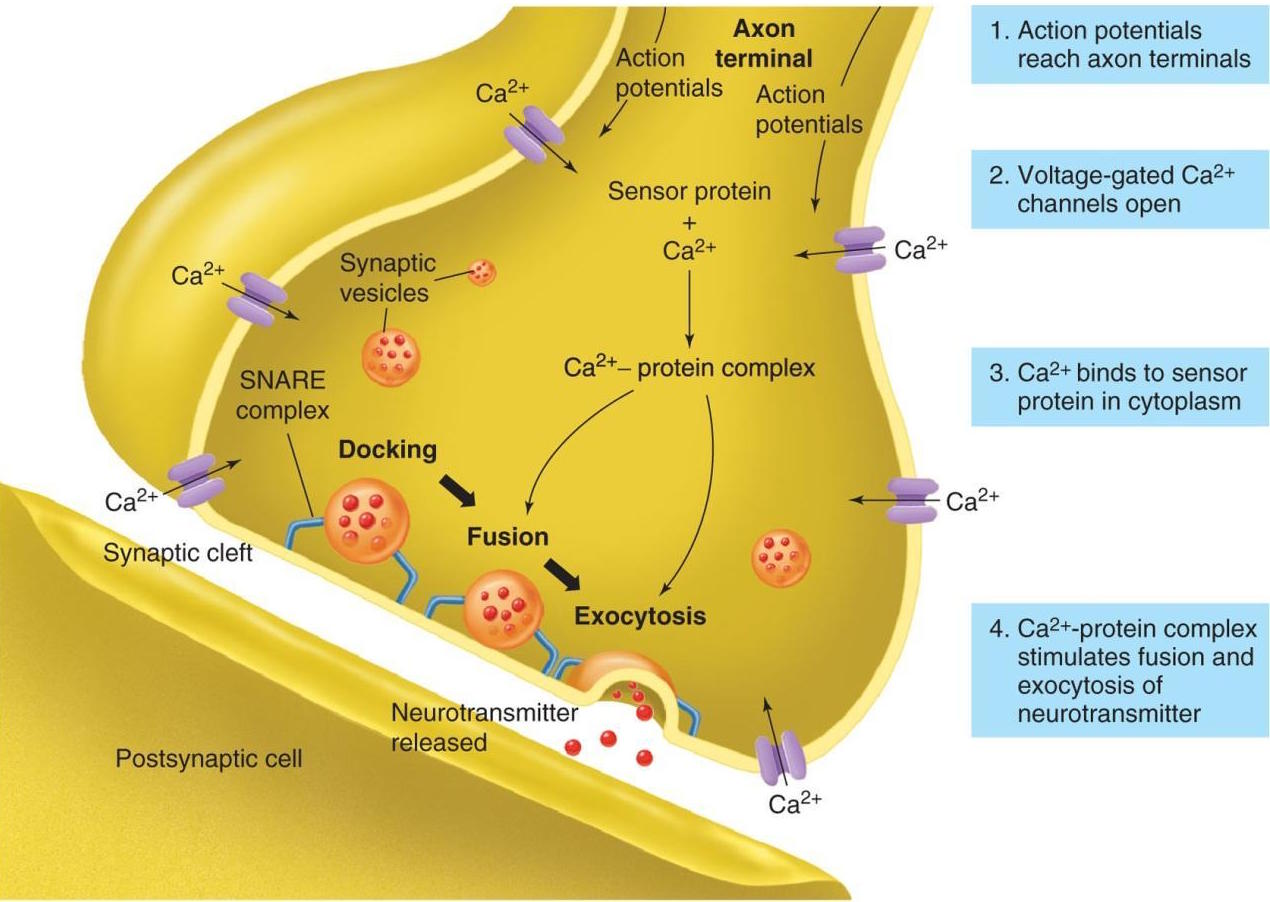
\includegraphics[width=1\textwidth]{fig1.jpg}
}


\begin{frame}{Synaptic Transmission}
\begin{columns}
\begin{column}{0.47\textwidth}
\begin{enumerate} \tiny
    \item<1->Action potential invades presynaptic cell and opens VGCCs
    \item<2->Calcium ions enter and activate SNAREpins in nerve terminal, causing vesicle fusion
    \item<3->Neurotransmitters (glutamate) diffuse across the cleft and bind to receptors (AMPA, NMDA)
    \item<4->Activated receptors allow for an influx of ions, produce a postsynaptic potential due to change in potential 
    \item<5->Excess neurotransmitter are taken up by glial cells to be reused
\end{enumerate}
    \end{column}
    \begin{column}{0.5\textwidth}
    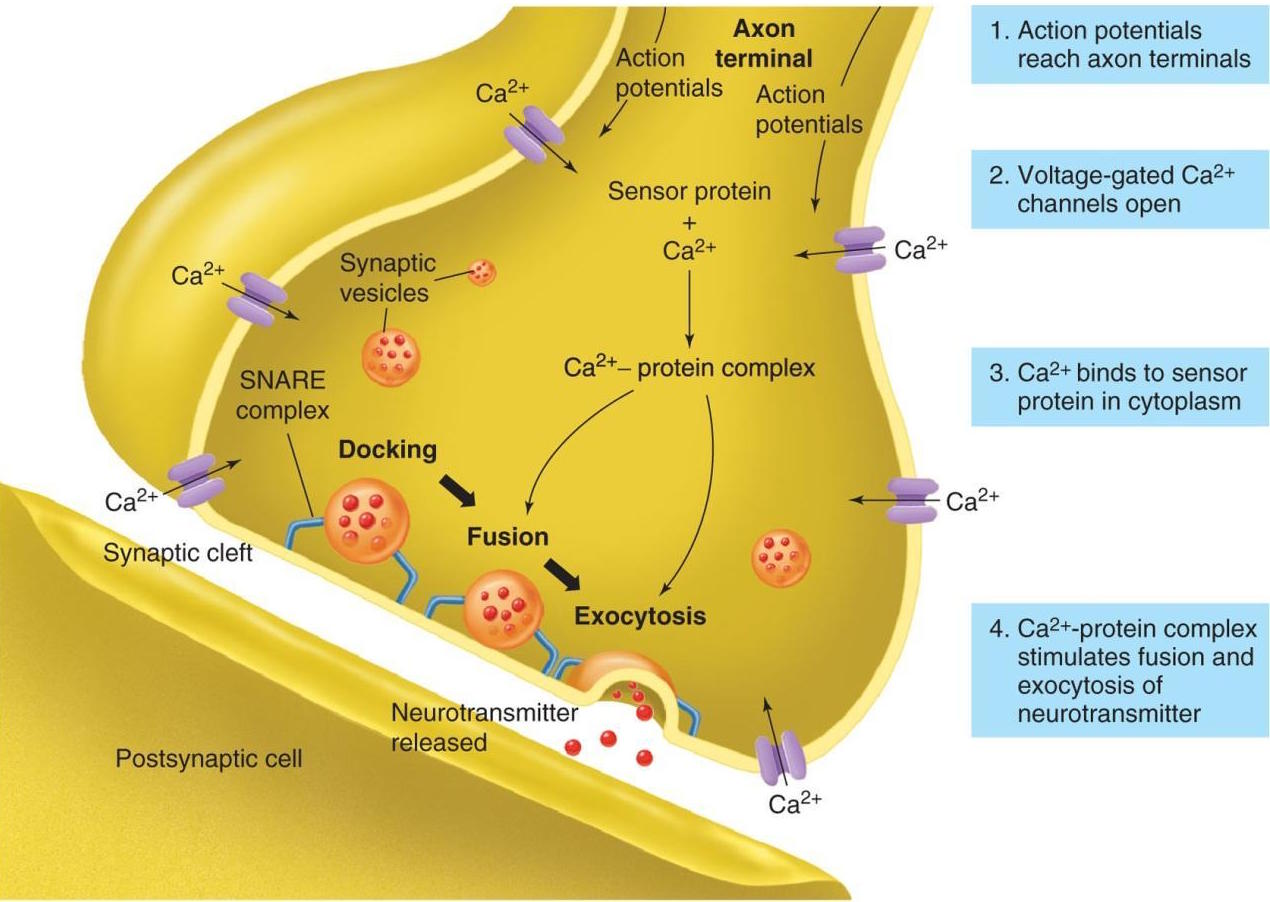
\includegraphics[width=1\textwidth]{fig1.jpg}
    \end{column}
\end{columns}
\end{frame}

\section{The Modelling Approach}
\frame
{
    \frametitle{Summary}
    Two phases - Phase I and Phase II
    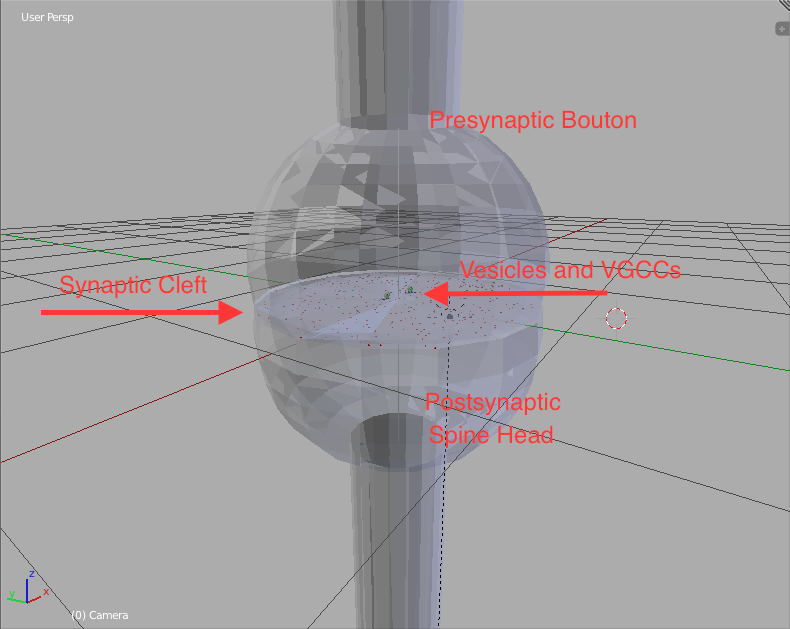
\includegraphics[width=1\textwidth]{fig2.png}
}

\frame
{
    \frametitle{Phase I}
    \begin{columns}
    \begin{column}{0.5\textwidth}
    \begin{itemize}
        \item Simulate calcium ion diffusion - but not the electrophysiology
        \item Simulate calcium binding to SNAREpins (Need two calcium to activate)
        \item Record time of vesicle fusion (require three activated SNAREpins on a vesicle)
    \end{itemize}
    \end{column}
    \begin{column}{0.5\textwidth}
    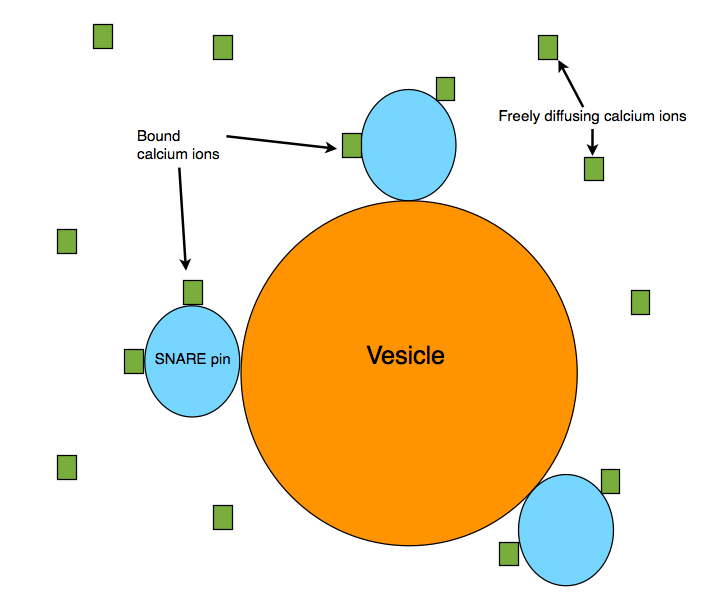
\includegraphics[width=1\textwidth]{presynaptic.png}
    \end{column}
\end{columns}
}

\frame
{
    \frametitle{Phase II}
    \begin{columns}
    \begin{column}{0.5\textwidth}
    \begin{itemize}
        \item Simulate diffusion of neurotransmitter across synaptic cleft 
        \item Simulate activation of neurotransmitter receptors 
    \end{itemize}
    \end{column}
\begin{column}{0.5\textwidth}
    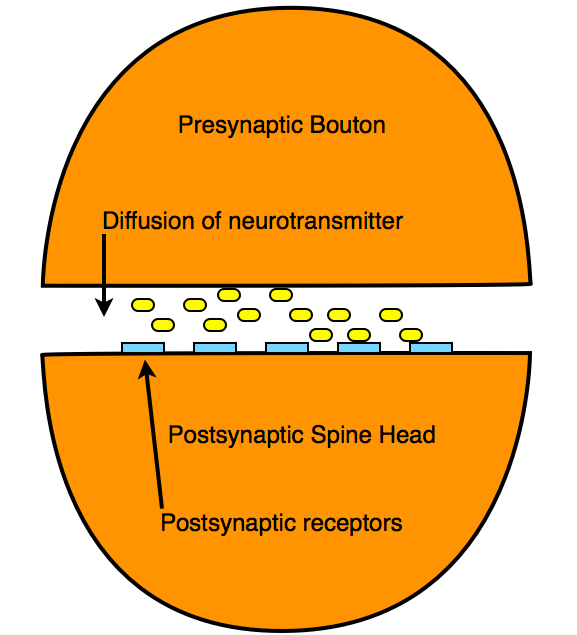
\includegraphics[width=1\textwidth]{postsynaptic.png}
    \end{column}
    \end{columns}
}

\frame
{ \frametitle{A question}
    \begin{itemize}
        \item Why not do everything in one step?
        \item The activation of SNAREpins is randomly determined during the simulation (depends on the movement of calcium ions)
        \item The release of neurotransmitter must be specified before the simulation is run (due to the way CellBlender defines molecule placement and release)
    \end{itemize}
}

\begin{frame}{Model Components}
\begin{columns}
\begin{column}{0.47\textwidth}
\begin{enumerate} 
    \item<1->Presynaptic bouton 
    \item<2->Spine head
    \item<3->Voltage-gated calcium channel regions (2)
    \item<4->Vesicles (2)
    \item<5->Glial cells
\end{enumerate}
    \end{column}
    \begin{column}{0.5\textwidth}
    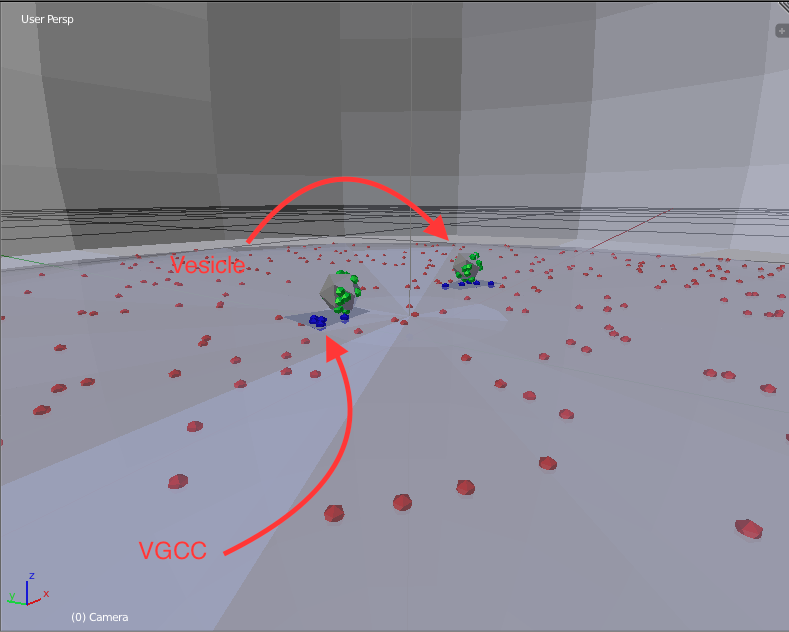
\includegraphics[width=1\textwidth]{fig3.png}
    \end{column}
\end{columns}
\end{frame}

\frame{
    \frametitle{Model Molecules}
\begin{enumerate}
    \item<1->VGCC - the calcium channels responsible for permitting flow of calcium into bouton. Has open and closed states.
    \item<2->Ca - calcium ion
    \item<3->CaBS - a SNARE complex which has no calcium ion bound
    \item<4->CaBS\_Ca - a SNARE complex which has one calcium ion bound
    \item<5->TAG - a SNARE complex which has two calcium ions bound
    \item<6->NT - a neurotransmitter molecule (represents glutamate)
    \item<7->LGIC - a neurotransmitter receptor residing on spine head (receptive to NT). Has open and closed states.
\end{enumerate}
}

\frame
{
\frametitle{Model Equations}
\begin{table}[H]
\begin{tabular}{ll}
Equation & Description \\ \hline
VGCC\_C $\to$ VGCC\_O & Calcium channel opening \\
VGCC\_O $\to$ VGCC\_C & Calcium channel closing \\
VGCC\_O $\to$ VGCC\_O + Ca & Calcium influx into bouton \\
Ca + CaBS $\to$ CaBS\_Ca & First calcium binding \\ 
CaBS\_Ca + Ca $\to$ TAG & Second calcium binding \\
NT + LGIC\_C $\to$ LGIC\_O& Neurotransmitter binding \\
\end{tabular} 
\end{table}

}

\section{Making the Model Realistic}
\frame
{
    \frametitle{Model Parameters}
    Need to calibrate:
    \begin{itemize}
        \item Rates
        \item Dimensions
        \item Quantities
    \end{itemize}
    to get a realistic model.
}

\frame
{
\frametitle{Model Rates}
\begin{table}[H]
\tiny
\begin{tabular}{ll}
Parameter & Value \\ \hline
Rate of calcium influx   &  $\SI{1e3}{\per\mole\litre\per\second}$      \\
SNARE complex binding rate & $\SI{1e8}{\per\mol\litre\per\second}$ \\
Glutamate binding rate & $\SI{4.6e6}{\per\mol\litre\per\second}$ \\
Rate of glutamate diffusion & $\SI{4e-6}{\centi\metre\squared\per\second} $      \\
Rate of calcium diffusion & $\SI{5.3e-6}{\centi\metre\squared\per\second} $      \\
Vesicle unzip time & \SI{200}{\micro\second}  \\
Estimate for bouton volume&  $\SI{0.36}{\micro\meter\cubed}$\\ 
Derived estimate for bouton radius & \SI{0.7}{\micro\meter} \\
Estimate for synaptic vesicle radius & $\SI{0.017}{\micro\meter}$ \\ 
Synaptic cleft width &$\SI{0.023}{\micro\meter}$\\
Number of Neurotransmitter molecules per vesicle & 4700\\
Number of Neurotransimtter receptors per spine head & 100 \\
Number of SNARE complexes per vesicle & 15 \\ 
Number of calcium ions to activate synaptotagmin/SNARE & 2 \\
Number of SNAREs to induce vesicle fusion & 3 \\  
Number of vesicles & 750 \\
\end{tabular}
\end{table}
}

\frame{
    \frametitle{Final Result}
    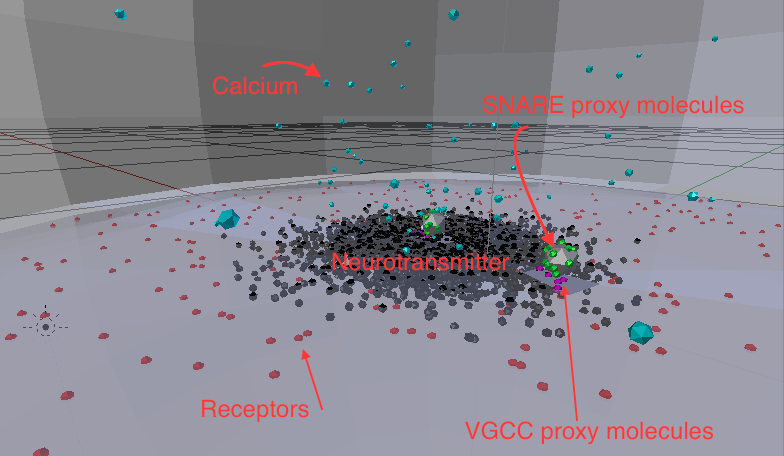
\includegraphics[width=1\textwidth]{legend.png}
}

\frame{
    \frametitle{Future Outlook}
    \begin{itemize}
        \item Improve model details - postsynaptic receptor, VGCCs
        \item Simulate the electrophysiology of the synapse
        \item Adapt model to different scenarios
    \end{itemize}

    
}
\frame{
    \frametitle{References}
    \begin{itemize}
        \item Synaptic terminal, obtained from https://classconnection.s3.amazonaws.com/811/flashcards/141811/jpg/synapse21329503162446.jpg
    \end{itemize}
}

\bibliography{report_doc}{}

\end{document}
